\documentclass[12pt]{article}

\usepackage{xspace}
\usepackage{lineno}
\usepackage{setspace}
\usepackage{graphicx}
\usepackage{subfigure}
\usepackage{float}
\usepackage{color}
\usepackage{caption}
\usepackage[margin=1in]{geometry}
\usepackage{epstopdf}
\usepackage{natbib}
\usepackage{amsmath}

\begin{document}
\doublespacing
\linenumbers


\newcommand{\LLik}{\ensuremath{\text{\emph{L}}}\xspace}


\noindent RH: LANDERER ET AL.--- Estimating genetic load
% put in your own RH (running head)
% for POVs the RH is always POINT OF VIEW
\bigskip
\medskip
\begin{center}

% Insert your title:
\noindent{\Large \bf Estimating the genetic load of natural protein coding sequences using a phylogenetic framework.}
\bigskip


\noindent{C\textsc{EDRIC} ~{L\textsc{ANDERER}}$^{1,2,*}$,
B\textsc{RIAN} C.~ {O\textsc{MEARA}}$^{1,2}$,
\textsc{AND}
M\textsc{ICHAEL} A.~{G\textsc{ILCHRIST}}$^{1,2}$}

\end{center}

\vfill

{\small
\noindent$^{1}$Department of Ecology \& Evolutionary Biology, University of Tennessee, Knoxville, TN 37996-1610\\
\noindent$^{2}$National Institute for Mathematical and Biological Synthesis, Knoxville, TN 37996-3410\\
\noindent$^{*}$Corresponding author. E-mail:~cedric.landerer@gmail.com
}

\vfill
\centerline{Version dated: \today}
\vfill
\newpage



\begin{abstract}
Protein production is a very costly process every cell performs, resulting in selection for proteins that can perform their function most efficiently.
The efficacy of selection is limited by the effective population size $N_e$, leading to genetic load via the introduction of mutations.
As all proteins have to face this selection-mutation-drift barrier, we expect to find proteins near a fitness peak, but never at the peak.
Here we assess the efficacy of selection on individual proteins and quantify the genetic load by phylogenetic inference of the optimal amino acid at each site using SelAC.
We demonstrate the assessment of the genetic load proteins impose for TEM in \textit{E. coli} and for cytochrome B in whales.
We quantify the genetic load for 49 TEM sequences and 12 cytochrome B sequences. 
We compare the inferred optimal TEM  amino acid sequence to fitness estimates from deep mutation scanning experiments.
We find that the observed TEM sequences have a 3 to 20 fold increased genetic load when compared to the DMS estimates instead of the SelAC inference.
Furthermore, we find that the DMS inference only shows 49 \% sequence agreement with the consensus sequence of the observed alignment.
We also observe a higher genetic load in CytB than in TEM, which is to be expected given the difference in $N_e$ between whales and \textit{E. coli}. 

\end{abstract}

\section*{Introduction}
\begin{itemize}
	\item Genetic load is a measure of distance between the average genotype's fitness and the genotype with the highest fitness.
	\begin{itemize}
		\item The genotype with the highest fitness is assed based on the set of observed genotypes.
		\item Mutation constantly introduces new, potentially deleterious mutations increasing the genetic load of a population.
		\item Genetic drift limits the efficacy of natural selection.
		\item Therefore, the optimal genotype is likely not among the observed genotypes.
		\item To remedy this, experimental procedures like deep mutation scanning can be employed to asses the fitness of genotypes.
	\end{itemize}
	\item Deep mutation scanning (DMS) requires a library of mutants for which the fitness should be assessed.
	\begin{itemize}
		\item This limits the application of DMS experiments to organisms that can be manipulated under laboratory conditions, and have a sufficiently short generation time.
		\item It also requires that artificial selection can be applied.
		\item This limits DMS experiments even further to proteins for which we can assume they respond to a singular stress factor.
		\item While it is save to ignore effects of mutation, the low population size does severely limit the efficacy of selection.
		\item It is therefore required to apply extremely strong selection pressure.
	\end{itemize}
	\item In this study, we assess how well DMS experiments can explain genetic load produced by natural evolution.
	\begin{itemize}
		\item It has previously been demonstrated that incorporation of DMS experiments into phylogenetic approaches improve model fit when compared to classical approaches like GY94.
		\item However, model adequacy has not been assessed.
		\item First we show that the models fits achieved by the incorporation of DMS experiments can be improved upon using a novel phylogenetic framework, SelAC.
		\item We compare the genetic load of natural TEM variants according to DMS and SelAC and show that DMS predicts an increased genetic load.
		\item We find that we would not expect to observe the natural TEM variants when simulating under the DMS inferred fitness landscape.
	\end{itemize}
	\item Having shown that SelAC provides more adequate inference of genetic load we further demonstrate its generality by assessing the genetic load of cytochrome B in whales.
\end{itemize}

\section*{Results}
\begin{itemize}
	\item We compared how well deep mutation scanning experiments can explain observed sequences and compared it to SelAC.
	\begin{itemize}
		\item We utilized DMS results from Stifler et al. for $\beta$-lactamase in E. coli. 
		\item We utilized phydms a tool designed to incorporate fitness estimates obtained from the DMS experiment into a phylogenetic framework.
		\item Model selection reveals that SelAC outperformes the the DMS experiment and better explains the observed sequences.
		\item Furthermore, we estimated the expected sequences given the fitness landscape described by DMS and SelAC.
		\begin{item}
			\item Simiulated sequences evolve to about 60 \% sequence similarity.
			\item We would also expect to observe less genetic load as sequences had time to evolve, assuming a reasonable $N_e$ of 1,000 or greater.
		\end{item}
	\end{itemize}
	\item We extimated the functionally optimal amino acid at each site from the observed sequence variation using SelAC.
	\begin{itemize}
		\item The observed TEM alignment shows a high percentage of homogeneous sites.
		\begin{itemize} 
			\item $68 \%$ of sites had only one codon present.
			\item $75 \%$ of sites encoded the same amino acid.
		\end{itemize}
		\item The observed CytB alignment shows a more codon heterogeneity but a similar homogeneity in amino acids.
		\begin{itemize} 
			\item $22 \%$ of sites had only one codon present.
			\item $78 \%$ of sites encoded the same amino acid.
		\end{itemize}
		\item We find that the predicted optimal amino acid sequence has high agreement with the observed consensus sequence of the alignment (TEM: $99 \%$, CytB: $95 \%$).
		\item In contrast, the experimentally obtained sequence estimate only has an agreement of $49 \%$ with the observed TEM consensus sequence.
		%\item Simulations based on the inferred optimal sequences showed that the we would not expect to the observed sequences to have evolved.
	\end{itemize}
	\item We assessed the genetic load of the observed sequences.
	\begin{itemize}
		\item We find that the genetic load of TEM differs greatly depending on the optimal amino acid sequence assumed.
		\begin{itemize}
			\item The genetic load of the observed sequences increases $3-20$ fold when using the experimentally inferred optimal sequence compared to the SelAC inferred optimal sequence.
			\item Besides the great variation that arises from the usage of different optimal amino acid sequences, we also find variation within each optimal amino acid sequence.
			\item E.g. $sN_e$ varies between $\sim0$ to $\sim-10$ for the SelAC optimal sequence and between $\sim -20$ to $\sim -27$ for the optimal sequence obtained from the DMS experiment.
		\end{itemize}
		\item We lack the ability to compare our estimates of genetic load for CytB as DMS experiment can not be performed on whales.
		\item We find a higher genetic load and greater variation in $sN_e$ for the CytB (not taken into account: sequences differ in length).
		\begin{itemize}
			\item $sN_e$ varies between $\sim -10$ to $\sim -35$.
		\end{itemize}
	\end{itemize}
	\item We are able to map variation in selection along the sequence and determine sites with higher contribution to genetic load.
	\begin{itemize}
		\item Increases in genetic load appear to be locally confined to a few regions among the TEM alignment but do not appear to be associated with any particular structural features.
		\item In contrast, CytB shows variation of genetic load across its whole sequence with a particularly strong increase in genetic load within the 5th transmembrane helix.
	\end{itemize}
	\item Previous work highlighted the advantages of DMS experiments for phylogenetic inferences.
	\item However, our estimates of genetic load of observed TEM sequences show that natural sequences would actually represent a large genetic load.
	\begin{itemize}
		\item The SelAC estimated optimal amino acid sequence outperformed the consensus sequence and the experimentally sequence explaining the data. 
		\item A second model selection was performed using phydms as an independent comparison.
		\begin{itemize}
			\item Model selection revealed that the main advantage of the DMS experiment comes from the fact that the input alignment is not needed to estimate amino acid preferences.
			\item While the experimentally inferred optimal sequence does a worse job explaining the observed sequences, model selection reveals that the improvement in likelihood does not justify the increased number of parameters required to run phydms with the SelAC or the consensus amino acid preferences.
		\end{itemize}
	\end{itemize}
\end{itemize}

\section*{Discussion}
\begin{itemize}
	\item We demonstrate the inference of site specific selection from protein coding sequence data using phylogenetics.
	\begin{itemize}
		\item We find that the fitness landscape estimated by SelAC better explains the observed sequences than DMS.
		\item Simulations show that the observed sequences would not arrise under the imposed selection during the DMS experiments.
		\item While DMS allows for the inferece of properties such as substitutions confering antibiotic resistance, it does not allow to explain natural sequence variation.
		\item In addition, as researrchers show more and more interests in non-model organisms, the limitation to proteins and organsism that can be manipulated under laboratory conditions limits its uses across the tree of life.
	\end{itemize}
	\item We estimate the genetic load of natural occurring proteins relative to an inferred optimal amino acid sequence.
	\item The optimal amino acid at each site was inferred from the observed proteins and their phylogenetic relationship.
	\item In both cases, TEM and CytB, we find high agreement between the consensus sequence inferred by ignoring the phylogenetic relationship and the optimal sequence inferred using SelAC (TEM: $99 \%$, CytB: $95 \%$).
	\begin{itemize}
		\item The strong agreement between consensus sequence and estimated optimal sequence for both proteins can be seen as an indication that the phylogenetic relationship does not play a large role in the examined cases.
		\item However, such an assumption should not be made a priory.
		\item The similarity between consensus and predicted optimal sequence could be because the proteins are under stabilizing selection like the model assumes, because rate of shifts in the optimal amino acid sequence is low, or because not enough time has passed for shifts to occur, despite diversifying selection.
		\item The used alignments contain a high amount of homogeneous sites (TEM: $ 75 \%$, CytB: $78 \%$), thus these sites do not allow for the inferred optimal amino acid to deviate from the observed consensus.
	\end{itemize}
	\item In contrast, the experimentally inferred optimal amino acid sequence for TEM only has $49 \%$ agreement with the observed consensus.
	\begin{itemize}
		\item Assuming that this inferred sequence is free of any bias introduced by the experimental conditions, we could only come to the conclusion that the observed TEM sequences show either strong mal-adaptation or did not have enough time to evolve towards the optimal sequence.
		\item However, \textit{E. coli} has a large effective population size, estimates are on the order of $10^8$ to $10^9$ (Ochman and Wilson 1987, Hartl et al 1994).
		\item The large $N_e$ would allow \textit{E. coli} to effectively "explore" the sequence space.
		\item On the other hand, each mutation in the library used for the DMS experiments starts of with only a few copies, potentially biasing the results due to strong genetic drift.
	\end{itemize}
	\item The genetic load of the observed sequences was inferred relative to the optimal amino acid sequence estimated by SelAC.
	\begin{itemize}
		\item Both, CytB and TEM show variation in the genetic load represented by each observed sequence, CytB represents a higher genetic load than TEM.
		\item Most TEM sequences show a small genetic load, likely due to the high selection pressure on TEM due to its usage in chemical warfare between microorganisms.
		\begin{itemize}
			\item If the experimental sequence is assumed to be most optimal, the observed TEM proteins represent a high genetic load to the organism. 
			\item This is would be in conflict with a large effective population size and therefore high efficacy of selection.
			\item However, while this would make fixation unlikely, it would not be impossible.
			\item In addition, the experimental sequence was inferred based on small population sizes for each genotype and artificial selection pressure. 
		\end{itemize}
	\end{itemize}
	\item Genetic load varies across the sequence.
	\begin{itemize}
		\item For both proteins, variation of $sN_e$ across the sequence is not associated with any particular structural features but mostly with variation in the alignment.
		\item However, TEM shows increased genetic load near the binding site, and the highest genetic load is found in the last beta sheet of the protein.
		\item The genetic load is generally higher for CytB than for TEM, and like for TEM genetic load appears to increase around the binding sites.
		\item However, for both proteins, increases in genetic load are not limited to the binding sites.
	\end{itemize}
	\item DMS experiments have been incorporated into phylogenetic studies to supplement information on selection on amino acids.
	\begin{itemize}
		\item In contrast, this study shows that information on selection can be extracted from alignments of protein coding sequences.
		\item To no surprise, model selection clearly favored the optimal sequence inferred by SelAC when using SelAC, however, when using this sequence in phydms we find that the inferences from SelAC still explained the data better, but the increase in parameters did not merit the increase in likelihood.
		\item This highlights the limitations of DMS sequences to explain natural evolution.
	\end{itemize}
\end{itemize}

\begin{table}
  \centering
  \begin{tabular}{lrrrr}
    Model	& \LLik &$n$ & AIC & $\Delta$AIC\\ \hline 
    SelAC	& -1498 & 374& 3744&  0\\
    SelAC+DMS 	& -1768 & 111& 3758& 14\\
    phyDMS 	& -2060 & 105& 4331& 586\\

  \end{tabular}
  \caption{\LLik, number of model parameters $n$, AIC, and $\Delta$AIC.}
  \label{tab:AIC}
\end{table}

\begin{figure}[h]
    \centering
    \begin{subfigure}
        \centering
        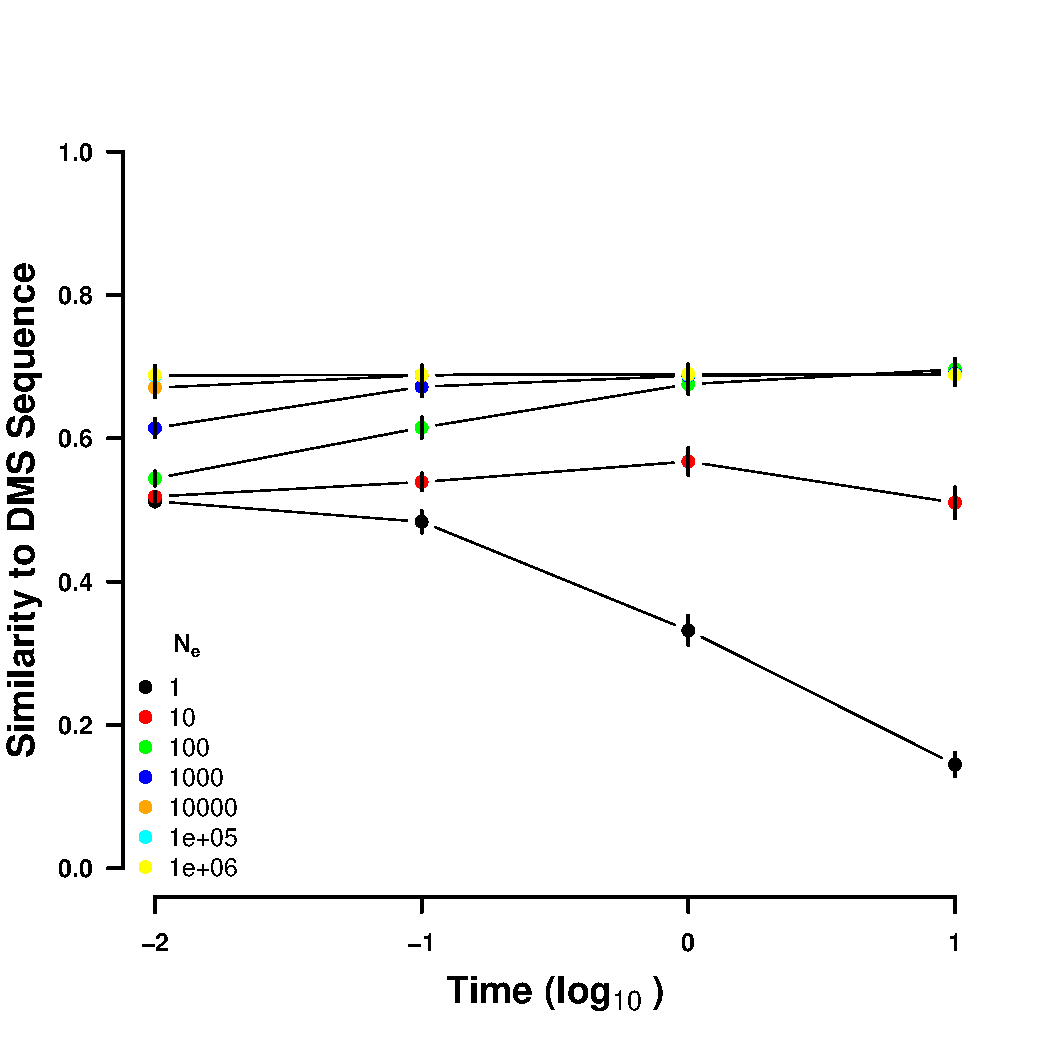
\includegraphics[width=.45\textwidth]{img/simulated_dist_time.pdf}
    \end{subfigure}
    \begin{subfigure}
        \centering
        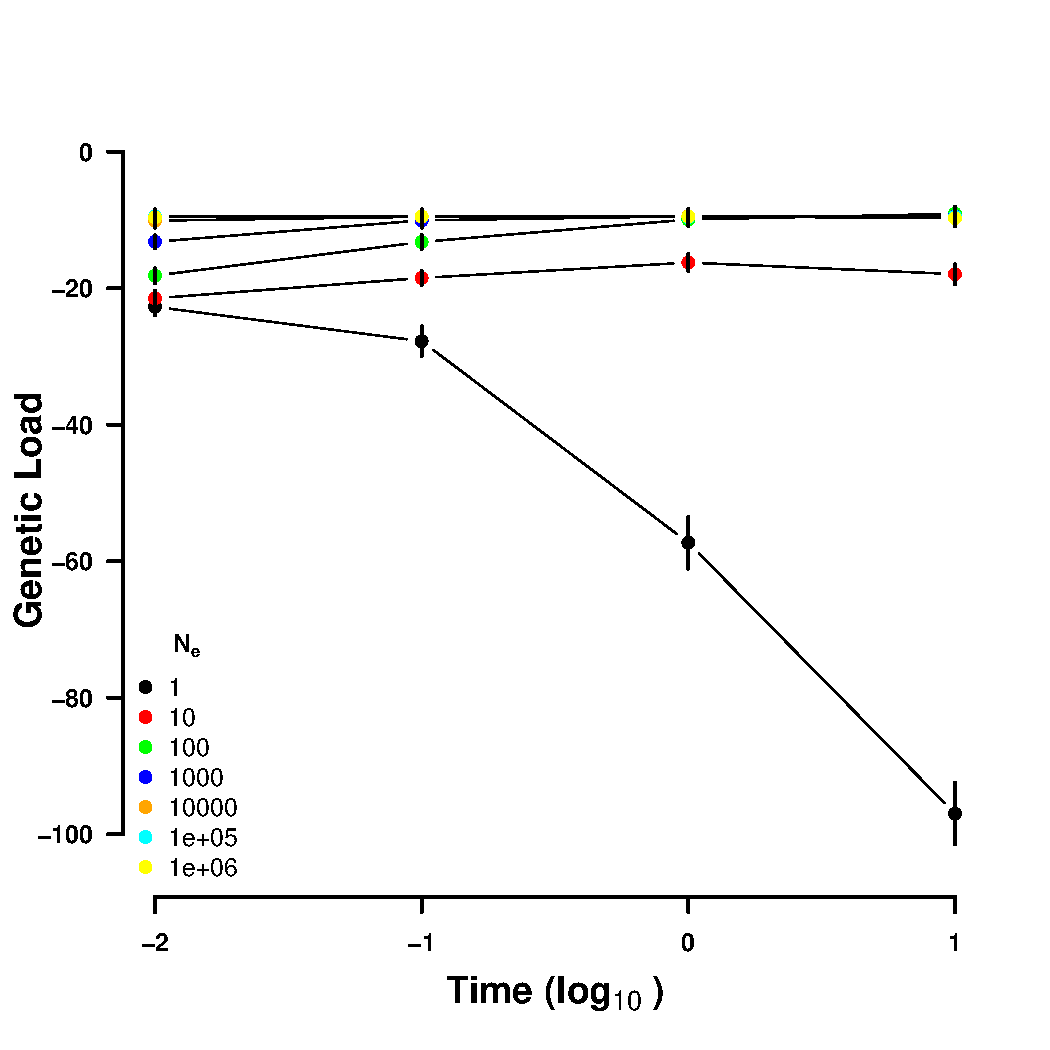
\includegraphics[width=.45\textwidth]{img/simulated_gl_time.pdf}
    \end{subfigure}
    \caption{Sequences simulated under various values of $N_e$ and for various times.}
    \label{fig:dms_sim}
\end{figure}

\begin{figure}[H]
     \centering
	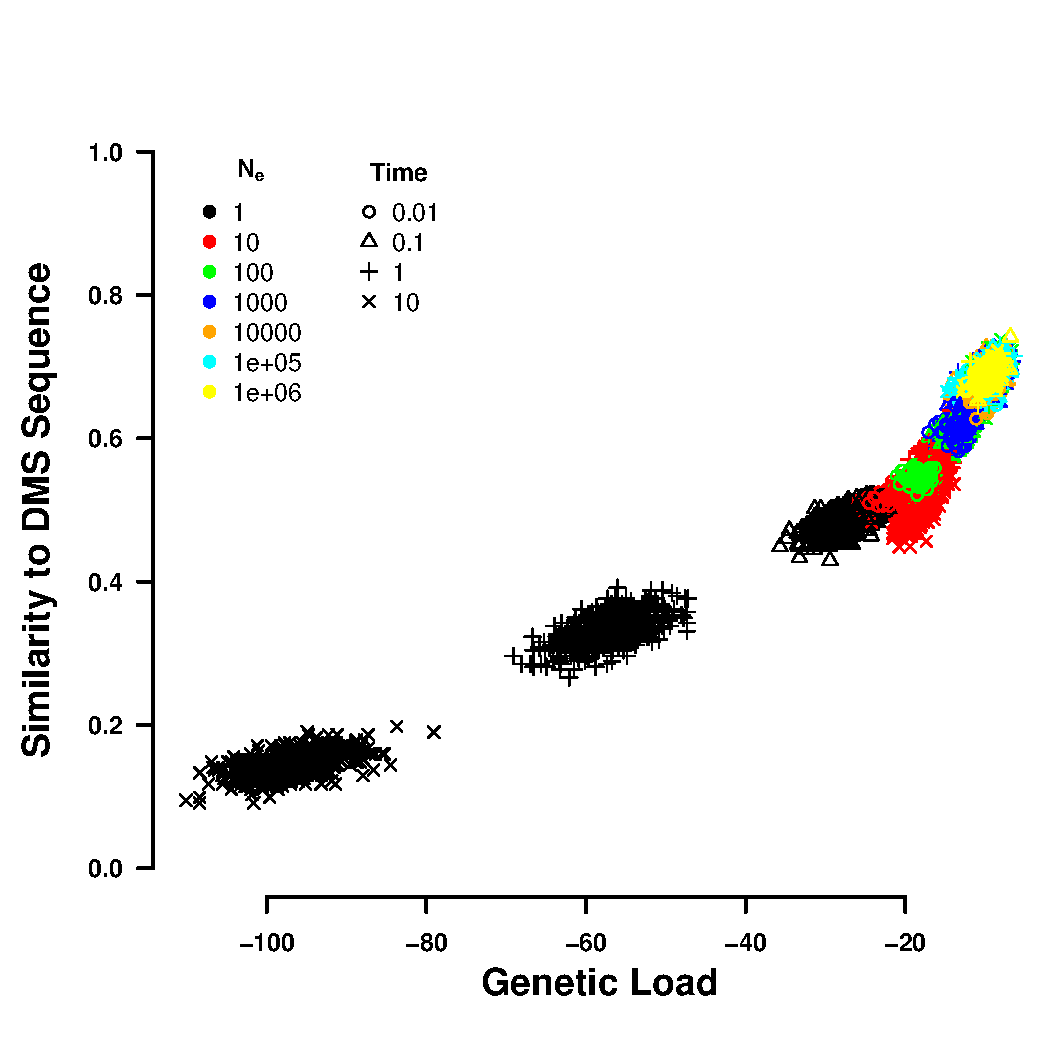
\includegraphics[width=0.6\textwidth]{img/simulated_seqs_gl_dist.pdf}
	\caption{Sequences simulated under various values of $N_e$ and for various times.}
	\label{fig:sim_seqs}
\end{figure}

\begin{figure}[H]
     \centering
	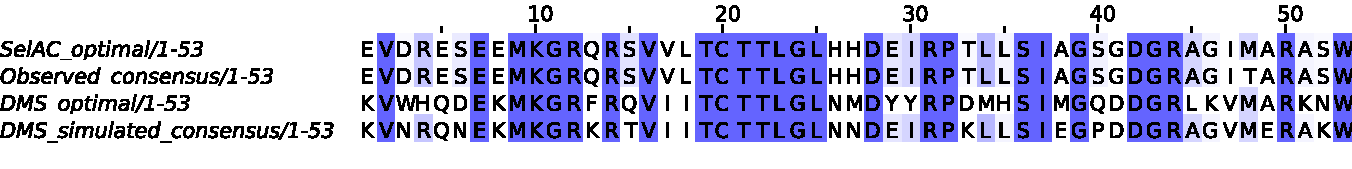
\includegraphics[width=\textwidth]{img/seq_simil_short.pdf}
	\caption{DMS and simulation based on DMS do not reflect natural sequences}
	\label{fig:sim_seqs_cons}
\end{figure}

\begin{figure}[h]
    \centering
    \begin{subfigure}
        \centering
        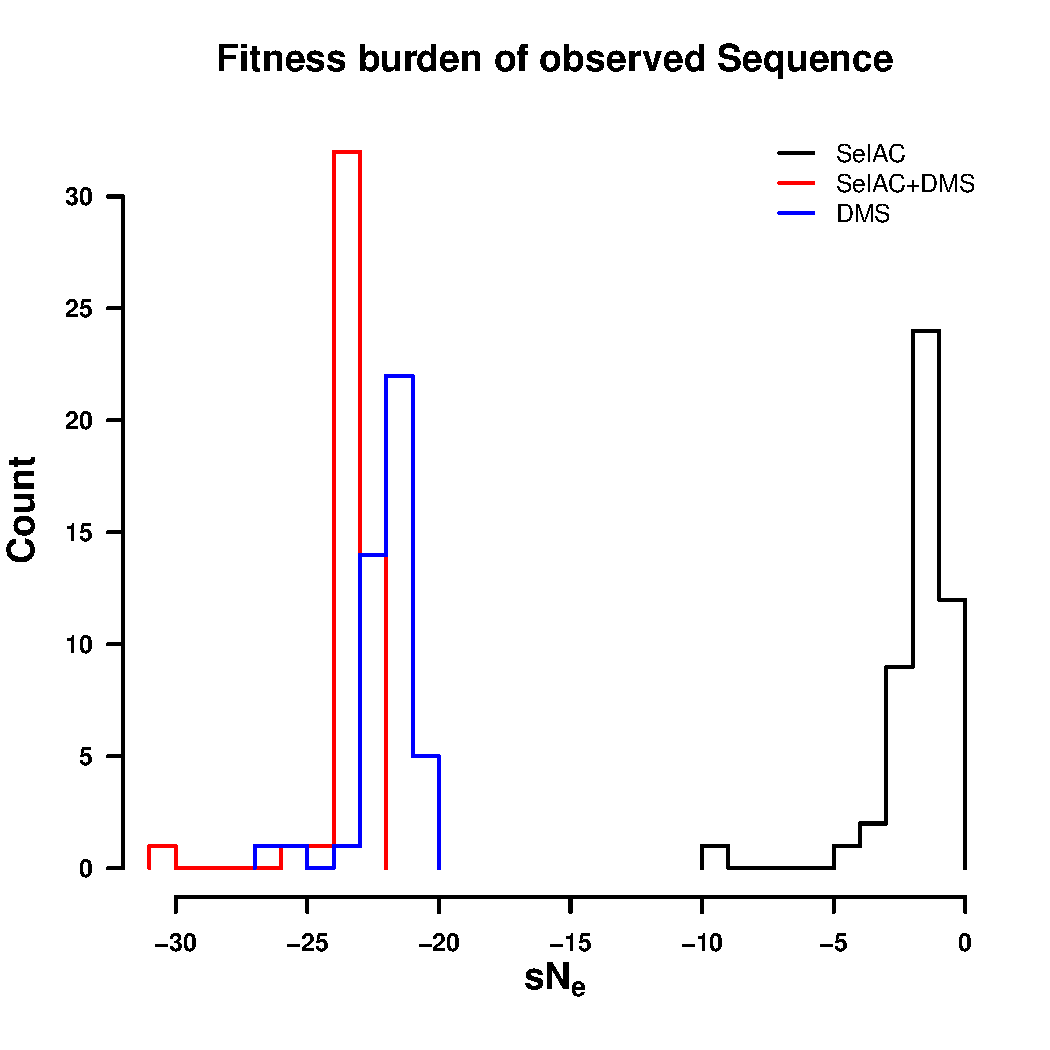
\includegraphics[width=.45\textwidth]{img/sNe_TEM2016.pdf}
    \end{subfigure}
    \begin{subfigure}
        \centering
        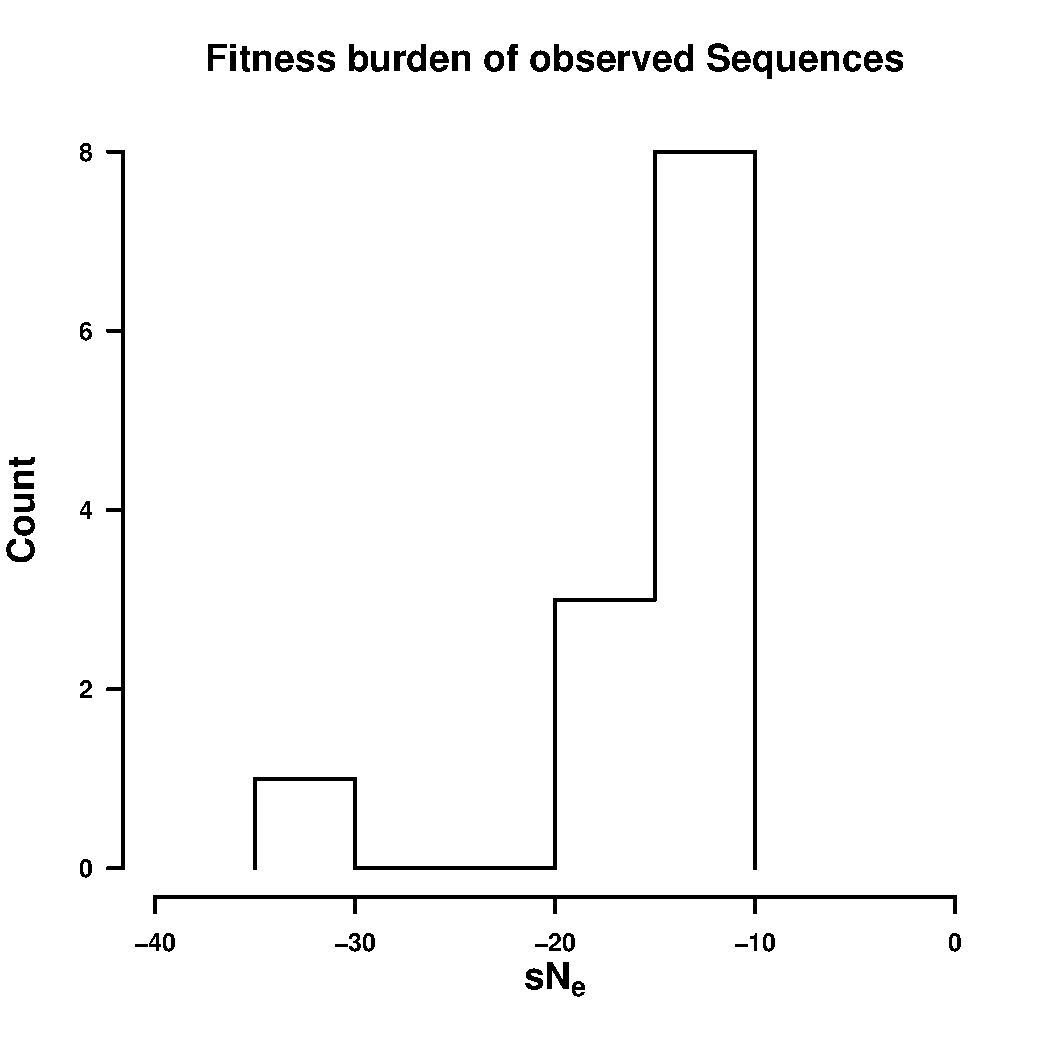
\includegraphics[width=.45\textwidth]{img/sNe_whale.pdf}
    \end{subfigure}
    \caption{$sN_e$ of whole sequence, variation across tips. TEM(left), CytB(right)}
    \label{fig:dms_sim}
\end{figure}



\begin{figure}[H]
     \centering
	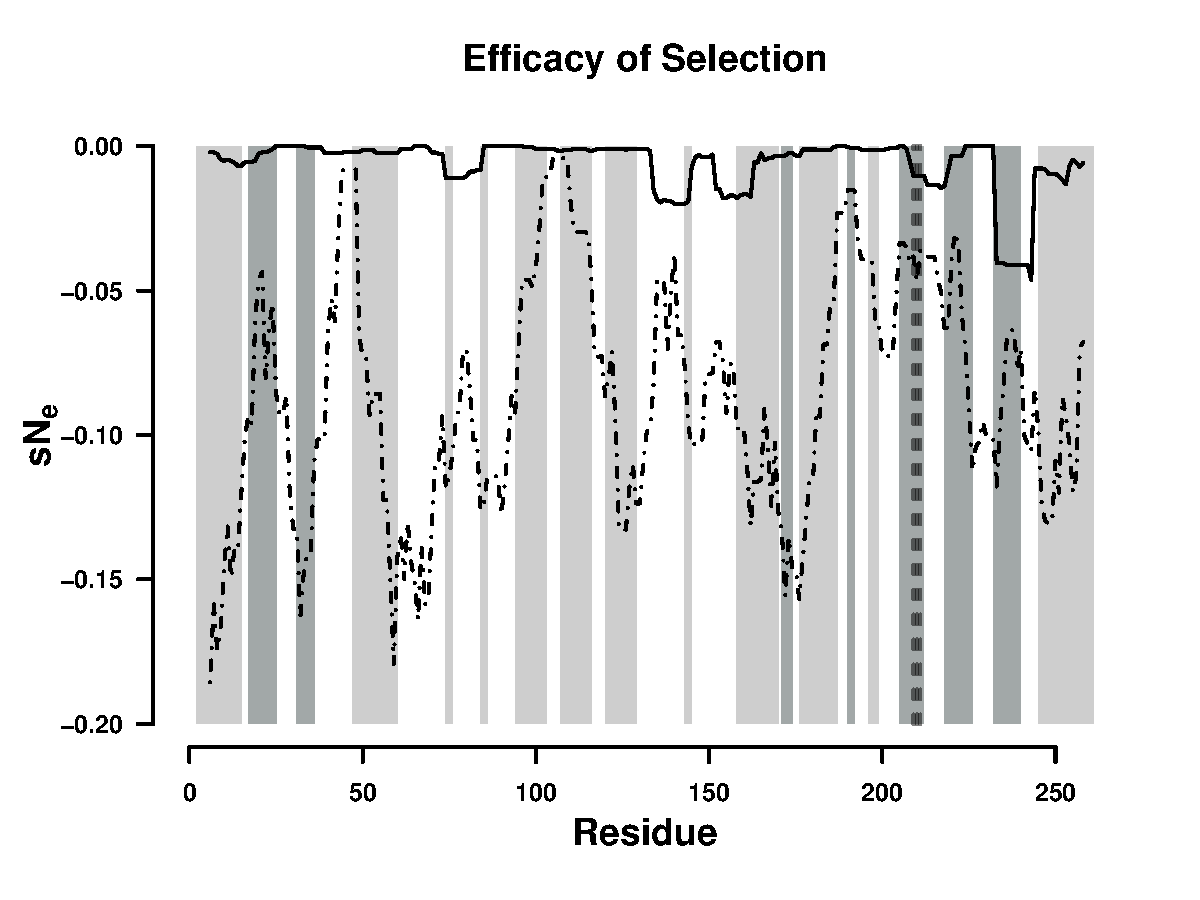
\includegraphics[width=\textwidth]{img/sNe_slide_TEM2016}
	\caption{TEM, bars are different seconday structure elements, dashed line is DMS sNe, solid is SelAC., horizontal lines are active/binding sites.}
	\label{fig:tem2016_sse}
\end{figure}

\begin{figure}[H]
     \centering
	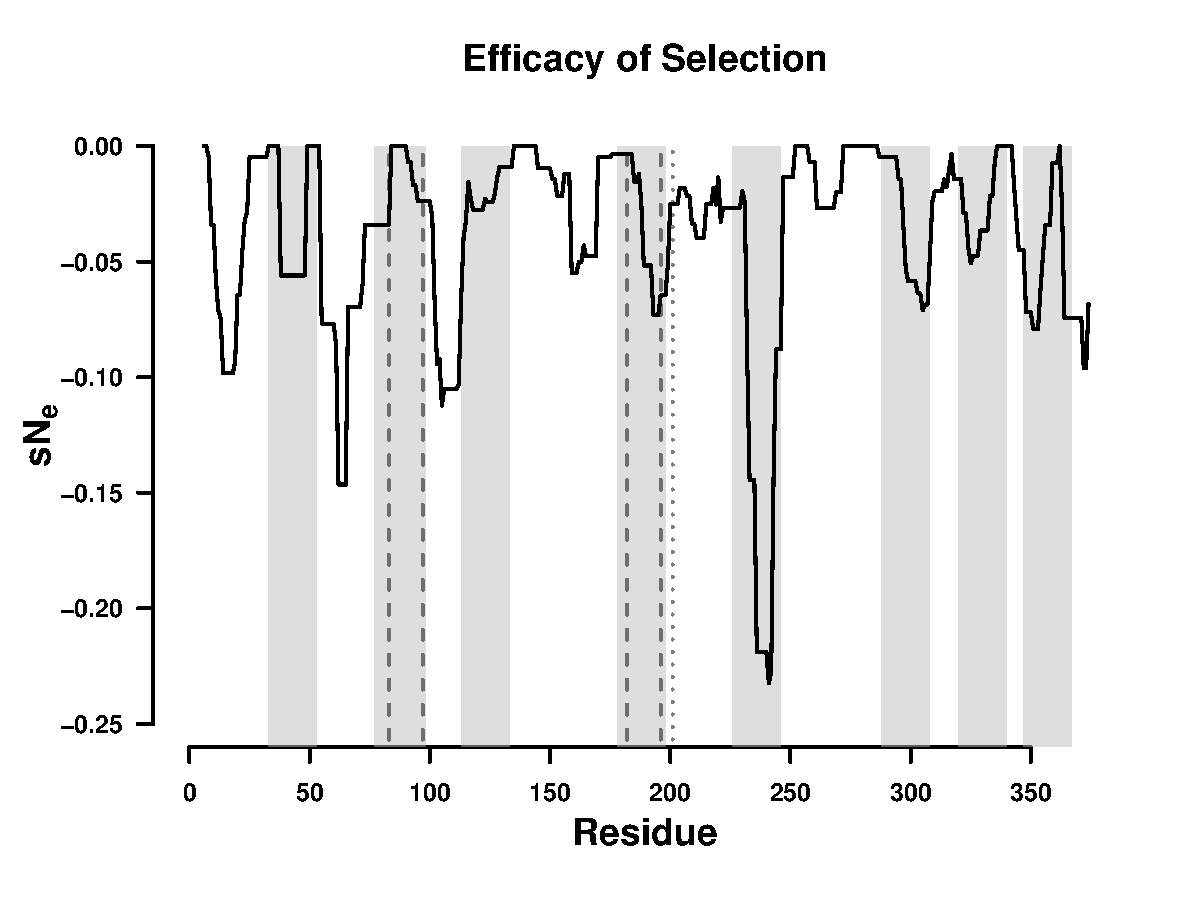
\includegraphics[width=\textwidth]{img/sNe_slide_whale}
	\caption{CytB}
	\label{fig:whale_sse}
\end{figure}

\end{document}







